\documentclass[a4paper,14pt]{extreport}
  \usepackage[left=1.5cm,right=1.5cm,
      top=1.5cm,bottom=2cm,bindingoffset=0cm]{geometry}
  \usepackage{scrextend}
  \usepackage[T1,T2A]{fontenc}
  \usepackage[utf8]{inputenc}
  \usepackage[english,russian,ukrainian]{babel}
  \usepackage{tabularx}
  \usepackage{amssymb}
  \usepackage{color}
  \usepackage{amsmath}
  \usepackage{mathrsfs}
  \usepackage{listings}
  \usepackage{graphicx}
  \graphicspath{ {./images/} }
  \usepackage{lipsum}
  \usepackage{xcolor}
  \usepackage{hyperref}
  \usepackage{tcolorbox}
  \usepackage{tikz}
  \usepackage{ulem}
  \usepackage[framemethod=TikZ]{mdframed}
  \usepackage{wrapfig,boxedminipage,lipsum}
  \mdfdefinestyle{MyFrame}{%
  linecolor=blue,outerlinewidth=2pt,roundcorner=20pt,innertopmargin=\baselineskip,innerbottommargin=\baselineskip,innerrightmargin=20pt,innerleftmargin=20pt,backgroundcolor=gray!50!white}
   \usepackage{csvsimple}
   \usepackage{supertabular}
  \usepackage{pdflscape}
  \usepackage{fancyvrb}
  %\usepackage{comment}
  \usepackage{array,tabularx}
  \usepackage{colortbl}
   \usepackage{fp}
   \usepackage{floatrow}
  \usepackage{varwidth}
  \tcbuselibrary{skins}
  \usepackage{fancybox}
  \usepackage{spreadtab}
   % Цвета для гиперссылок
  \definecolor{linkcolor}{HTML}{799B03} % цвет ссылок
  \definecolor{urlcolor}{HTML}{799B03} % цвет гиперссылок


  \usepackage{tikz}
  \usepackage[framemethod=TikZ]{mdframed}
  \usepackage{xcolor}
  \usetikzlibrary{calc}
  \makeatletter
  \newlength{\mylength}
  \xdef\CircleFactor{1.1}
  \setlength\mylength{\dimexpr\f@size pt}
  \newsavebox{\mybox}
  \newcommand*\circled[2][draw=blue]{\savebox\mybox{\vbox{\vphantom{WL1/}#1}}\setlength\mylength{\dimexpr\CircleFactor\dimexpr\ht\mybox+\dp\mybox\relax\relax}\tikzset{mystyle/.style={circle,#1,minimum height={\mylength}}}
  \tikz[baseline=(char.base)]
  \node[mystyle] (char) {#2};}
  \makeatother

  \definecolor{ggreen}{rgb}{0.4,1,0}
  \definecolor{rred}{rgb}{1,0.1,0.1}
  \definecolor{amber}{rgb}{1.0, 0.75, 0.0}
  \definecolor{babyblue}{rgb}{0.54, 0.81, 0.94}
  \definecolor{amethyst}{rgb}{0.6, 0.4, 0.8}

  \usepackage{float}
  \usepackage{wrapfig}
  \usepackage{framed}
  %for nice Code{
  \lstdefinestyle{customc}{
    belowcaptionskip=1\baselineskip,
    breaklines=true,
    frame=L,
    xleftmargin=\parindent,
    language=C,
    showstringspaces=false,
    basicstyle=\small\ttfamily,
    keywordstyle=\bfseries\color{green!40!black},
    commentstyle=\itshape\color{purple!40!black},
    identifierstyle=\color{blue},
    stringstyle=\color{orange},
  }
  \lstset{escapechar=@,style=customc}
  \usepackage{multicol}
  \usepackage{caption}
  \usepackage{subcaption}
  \usepackage{stfloats} % for positioning of figure* on the same page
  
  
  
%}


\begin{document}
  \pagecolor{white}

  %----------------------------------------1
  \newtcbox{\xmybox}[1][red]{on line, arc=7pt,colback=#1!10!white,colframe=#1!50!black, before upper={\rule[-3pt]{0pt}{10pt}},boxrule=1pt, boxsep=0pt,left=6pt,right=6pt,top=2pt,bottom=2pt}

  \begin{titlepage}
    \begin{center}
      \large
      Національний технічний університет України \\ "Київський політехнічний інститут імені Ігоря Сікорського"


      Факультет Електроніки

      Кафедра мікроелектроніки
      \vfill

      \textsc{ЗВІТ}\\

      {\Large Про виконання лабораторної роботи №3\\
        з дисципліни: «Фізичні основи сенсорики»\\[1cm]

         Оптичні сенсори газу (рідини)


      }
    \bigskip
  \end{center}
  \vfill

  \newlength{\ML}
  \settowidth{\ML}{«\underline{\hspace{0.4cm}}» \underline{\hspace{2cm}}}
  \hfill
  \begin{minipage}{1\textwidth}
  Виконавець:\\
  Студент 4-го курсу \hspace{4cm} $\underset{\text{(підпис)}}{\underline{\hspace{0.2\textwidth}}}$  \hspace{1cm}А.\,С.~Мнацаканов\\
  \vspace{1cm}

  Перевірив: \hspace{6.1cm} $\underset{\text{(підпис)}}{\underline{\hspace{0.2\textwidth}}}$  \hspace{1cm}ас. Коваль В. М.\\

  \end{minipage}

  \vfill

  \begin{center}
  2021
  \end{center}
\end{titlepage}



\newpage
\setcounter{page}{2}
\textbf{Мета роботи} – за допомогою інфрачервоного сенсору дослідити стан свого подиху та шкіри.


\begin{center}
\textbf{Порядок виконання роботи}
\end{center}
\begin{enumerate}
  \item Ввімкнути джерело постійного струму ИПТ Б5-49, виставити вихідну
  напругу 3 В.
  \item  Виміряти передаточну характеристику ІЧ-сенсору газу – залежність
  вихідного струму сенсора від струму на його вході. Вхідний струм
  змінювати в межах 5...80 мА з кроком 5 мА. На передаточній
  характеристиці обрати робочу точку сенсора.
  \item  Дослідити кінетику десорбції парів газу, адсорбованого на робочій поверхні
  призми ІЧ-сенсора під час видоху людини. При цьому кожному студенту
  підгрупи пропонується вивчити стан свого подиху шляхом вимірювання за
  допомогою мікроамперметра М2027 та таймера залежності вихідного струму сенсору від часу в процесі десорбції. Після кожного вимірювання
  робочу поверхню призми ІЧ-сенсора потрібно ретельно очищати.
  \item Вивчити стан шкіри кожного із студентів підгрупи за допомогою ІЧ-сенсора. Для цього потрібно виміряти за допомогою мікроамперметра М2027 відхилення струму сенсора від робочої точки при дотику пальцем до його робочої поверхні. Після кожного вимірювання робочу поверхню призми ІЧ-сенсора потрібно ретельно очищати.
  \item  Вимкнути джерело постійного струму ИПТ Б5-49.
\end{enumerate}

\clearpage
\newpage

\begin{center}
\textbf{Результати роботи}
\end{center}

%-------------------------------------
Тепер за допомогою знятих даних з лабораторних приладів, складемо таблиці та на їх основі побудуємо графіки. 
\begin{figure}[h]
\begin{minipage}{.45\textwidth}
  \centering
   \subcaption{Дані для передаточної характеристики ІЧ-сенсору газу.}
  \begin{tabular}{|c|c|}\hline
    $I_{\text{вх}}$, мА & $I_{\text{вих}}$, мкА \\ \hline
    10                & 8                  \\ \hline
    20                & 19                 \\ \hline
    30                & 32                 \\ \hline
    40                & 43                 \\ \hline
    50                & 54                 \\ \hline
    60                & 65                 \\ \hline
    70                & 75                 \\ \hline
    80                & 85                 \\ \hline
    90                & 95                 \\ \hline
    \end{tabular}
\end{minipage}\hfill
\begin{minipage}{.55\textwidth}
  \centering 
  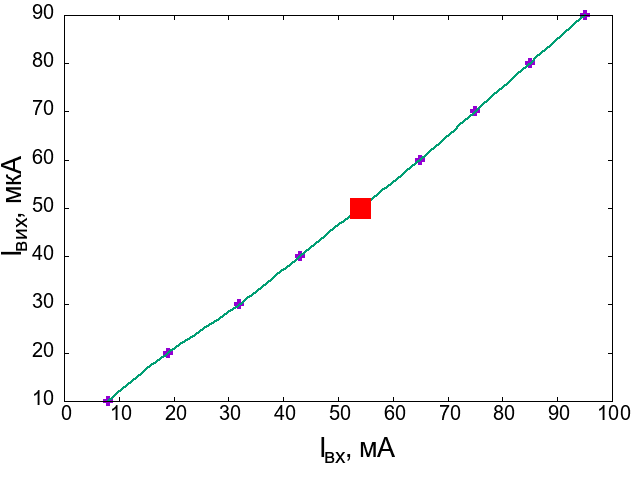
\includegraphics[width=0.8\textwidth]{1.png}
  \subcaption{Передаточна характеристика ІЧ-сенсору газу з позначеної на ній робочою точкою сенсора.}
\end{minipage}
\caption{}
\end{figure}

\vspace{0.1cm}
\noindent\rule{\textwidth}{1pt}
\vspace{0.1cm}

\begin{figure}[h]
\begin{minipage}{.45\textwidth}
  \centering
   \subcaption{Дані для графіку часової залежності процесу десорбції подиху кожного студента №1}
   \label{ris2a}
  \begin{tabular}{|c|c|}
    \hline
    $I_{\text{вих}}$,мкА & t, c \\ \hline
    45                 & 0    \\ \hline
    47                 & 1    \\ \hline
    49                 & 2    \\ \hline
    51                 & 3    \\ \hline
    53                 & 4    \\ \hline
    55                 & 5    \\ \hline
  \end{tabular}
\end{minipage}\hfill
\begin{minipage}{.55\textwidth}
  \centering 
  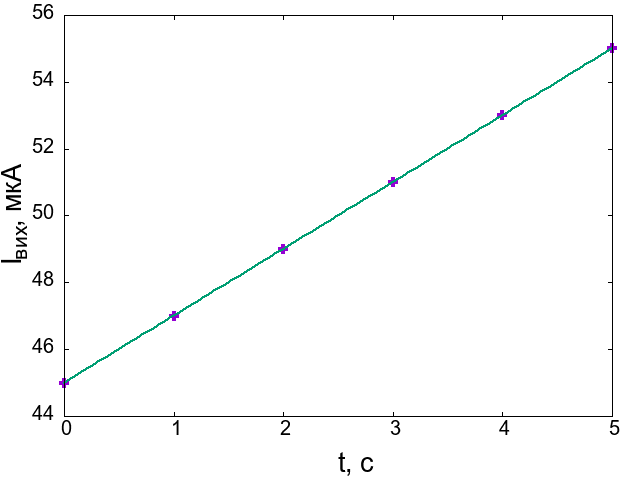
\includegraphics[width=0.8\textwidth]{2.png}
  \subcaption{Графік часової залежності процесу десорбції подиху кожного студента №1}
  \label{ris2b}
\end{minipage}
\caption{}
\end{figure}
 
\begin{figure}[h]
\begin{minipage}{.45\textwidth}
  \centering
   \subcaption{Дані для графіку часової залежності процесу десорбції подиху кожного студента №2}
   \label{ris3a}
  \begin{tabular}{|c|c|}
    \hline
    $I_{\text{вих}}$,мкА & t, c \\ \hline
    42                 & 0    \\ \hline
    45                 & 1    \\ \hline
    46                 & 2    \\ \hline
    47                 & 3    \\ \hline
    48                 & 4    \\ \hline
    49                 & 5    \\ \hline
  \end{tabular}
\end{minipage}\hfill
\begin{minipage}{.55\textwidth}
  \centering 
  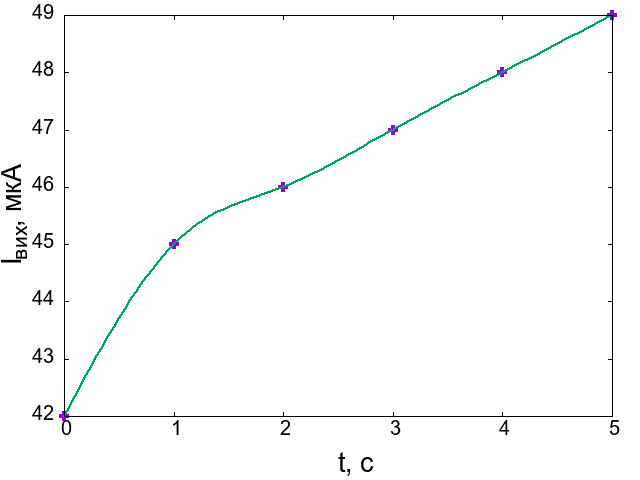
\includegraphics[width=0.8\textwidth]{lexa.png}
  \subcaption{Графік часової залежності процесу десорбції подиху кожного студента №2}
  \label{ris3b}
\end{minipage}
\caption{}
\end{figure}

\texttt{Дивлячись на Рис.\ref{ris2a}  та Рис.\ref{ris3a} можна стверджувати, що у студента №1 \\ десорбція парів газу (подиху) з поверхні призми проходить швидше - це \\пояснюється тим, що у студента №1 в подиху налічується більше летких \\ речови, ніж у студента №2.}





\begin{tcolorbox}[colback=white!100,colframe=red!95!black,width=19cm,righttitle=0.5cm,subtitle style={boxrule=0.4pt, colback=yellow!50!red!25!white},title= \bf{\texttt{студент №1}}\hfill  \bf{\texttt{студент №2}}]
  \begin{center}\bf{$I_{\text{вих}}$ = 42 мкА}\hfill  \bf{$I_{\text{вих}}$ = 36 мкА}\end{center}
  \tcblower
  \bf{$\triangle = 54-42 = 12$}\hfill  \bf{$\triangle = 54-36 = 18$}
\end{tcolorbox}

\vspace{1cm}
\texttt{Дивлячись на  дані зазначені вище, можна зробити висновок, що студент №2 має більше адсорбційних центрів ніж №1, тобто його стан шкіри більш \\ забруднений \sout{або він просто сильніше натиснув на призму}}.










\newpage
\clearpage
\vspace{5cm}
\begin{center}
\textbf{Контрольні запитання}
\end{center}
\begin{enumerate}
\item На чому ґрунтуються оптичні методи вимірювання концентрації та складу
газової суміші?
\item  Які параметри електромагнітної хвилі змінюються при проходженні крізь
простір з рівномірним розподілом досліджуваної речовини?
\item  Які Ви знаєте різновидності оптичних методів вимірювання концентрації та
складу газової суміші?
\item  В чому полягає рефрактометричний метод аналізу газової суміші?
\item  Який закон лежить в основі поляриметричного методу аналізу речовини?
\item  На чому ґрунтується нефелометричний метод аналізу газової суміші?
Вкажіть області його застосування.
\item  В чому полягає колориметричний метод аналізу речовини?
\item  Поясніть фізичну суть спектрального методу аналізу газів та рідин.
\item  Що таке абсорбційна спектроскопія? Яке її практичне значення?
\item  Напишіть математичний вираз закону Ламберта-Бугера-Берра. Який його
фізичний зміст?
\end{enumerate}


\end{document}